% Copyright 2006 by Till Tantau
%
% This file may be distributed and/or modified
%
% 1. under the LaTeX Project Public License and/or
% 2. under the GNU Free Documentation License.
%
% See the file doc/generic/pgf/licenses/LICENSE for more details.


\section{Arrow Tip Library}
\label{section-library-arrows}

\begin{pgflibrary}{arrows}
  The package defines additional arrow tips, which are described
  below. Note that neither the standard packages nor
  this package defines an arrow name containing |>| or |<|. These are
  left for the user to defined as he or she sees fit.
\end{pgflibrary}

The arrow tips |to|, |stealth|, |latex|, |space|, their reversed
forms, and \verb!|! are predefined, but listed below for completeness,
nevertheless. 


\subsection{Mathematical Arrow Tips}

\begin{tabular}{ll}
  \symarrow{to} \\
  \symarrow{to reversed} \\
  \symarrowdouble{implies} \\
\end{tabular}


\subsection{Triangular Arrow Tips}

\begin{tabular}{ll}
  \symarrowdouble{latex} \\
  \symarrowdouble{latex reversed}  \\
  \symarrow{latex'} \\
  \symarrow{latex' reversed}  \\
  \symarrowdouble{stealth} \\
  \symarrowdouble{stealth reversed}  \\
  \symarrow{stealth'} \\
  \symarrow{stealth' reversed}\\
  \symarrow{triangle 90} \\
  \symarrow{triangle 90 reversed}   \\
  \symarrow{triangle 60} \\
  \symarrow{triangle 60 reversed}   \\
  \symarrow{triangle 45} \\
  \symarrow{triangle 45 reversed}   \\
  \symarrow{open triangle 90} \\
  \symarrow{open triangle 90 reversed}   \\
  \symarrow{open triangle 60} \\
  \symarrow{open triangle 60 reversed}   \\
  \symarrow{open triangle 45} \\
  \symarrow{open triangle 45 reversed}   \\
\end{tabular}


\subsection{Barbed Arrow Tips}

\begin{tabular}{ll}
  \symarrow{angle 90} \\
  \symarrow{angle 90 reversed}   \\
  \symarrow{angle 60} \\
  \symarrow{angle 60 reversed}   \\
  \symarrow{angle 45} \\
  \symarrow{angle 45 reversed}   \\
  \symarrow{hooks} \\
  \symarrow{hooks reversed} \\
\end{tabular}


\subsection{Bracket-Like Arrow Tips}

{
\bigskip
\catcode`\|=12
\begin{tabular}{ll}
  \sarrow{[}{]} \\
  \sarrow{]}{[} \\
  \sarrow{(}{)} \\
  \sarrow{)}{(} \\
  \index{*vbar@\protect\texttt{\protect\myvbar} arrow tip}%
  \index{Arrow tips!*vbar@\protect\texttt{\protect\myvbar}}
  \texttt{\char`\|-\char`\|} & yields thick  
  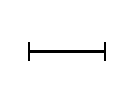
\begin{tikzpicture}[arrows={|-|},thick]
    \useasboundingbox (0pt,-0.5ex) rectangle (1cm,2ex);
    \draw (0,0) -- (1,0);
  \end{tikzpicture} and thin
  \begin{tikzpicture}[arrows={|-|},thin]
    \useasboundingbox (0pt,-0.5ex) rectangle (1cm,2ex);
    \draw (0,0) -- (1,0);
  \end{tikzpicture}
\end{tabular}
}

\subsection{Circle, Diamond and Square Arrow Tips}


\begin{tabular}{ll}
  \symarrow{o} \\
  \symarrow{*} \\
  \symarrow{diamond} \\
  \symarrow{open diamond}   \\
  \symarrow{square} \\
  \symarrow{open square}   \\
\end{tabular}



\subsection{Serif-Like Arrow Tips}

\begin{tabular}{ll}
  \symarrow{serif cm}
\end{tabular}


\subsection{Partial Arrow Tips}

\begin{tabular}{ll}
  \symarrow{left to} \\
  \symarrow{left to reversed} \\
  \symarrow{right to} \\
  \symarrow{right to reversed} \\
  \symarrow{left hook} \\
  \symarrow{left hook reversed} \\
  \symarrow{right hook} \\
  \symarrow{right hook reversed}
\end{tabular}



\subsection{Line Caps}

\begin{tabular}{ll}
  \carrow{round cap} \\
  \carrow{butt cap} \\
  \carrow{triangle 90 cap} \\
  \carrow{triangle 90 cap reversed} \\
  \carrow{fast cap} \\
  \carrow{fast cap reversed} \\
\end{tabular}


\subsection{Spacing Tips}

The spacing arrow tips are useful for combining them with other arrows
to get arrows that do not touch the end of the line.

\begin{tabular}{ll}
  \symarrow{space} \\
\end{tabular}


%%% Local Variables: 
%%% mode: latex
%%% TeX-master: "pgfmanual-pdftex-version"
%%% End: 
